\documentclass[10pt]{article}
\usepackage{geometry, graphicx}
\geometry{letterpaper}                 

\title {Lab Report 1 Submission (2019)}
\author{Sylvain Lapeyrade, Reda Bourakkadi\, (sylla801, redbo196)}
\begin{document}
\maketitle

\section*{Answers}

\subsection*{1) \textbf{ Exercise 1: Coalition structure generation}}
\textit {You should plot and discuss your results in the report—e.g.,
 what is the solution quality of the different algorithms,
  and what type of problems are they suitable for?} \medskip

 After implementing both the random and greedy search algorithms, we obtained
  the results detailed in Figure \ref{fig:csg_data}. We can see at first view
  that the \textbf{Greedy Search} algorithm does not find the best utility value for each
  problem and for each number of agents which is respectively 15 for problems 1 and 2,
  and 20 for problems 3 and 4. \medskip

 Indeed, for the problem 1, the \textbf{Greedy Search} is a bit lower than the 
  \textbf{Random Search} value with 10 000 and 100 000 evaluations (i.e. 7.8364 $>$ 
  8.22902 $>$ 8.65678). However, for the problem 2, the tendency is inverted (i.e. Random
  Search with 100 000 evals: 9.11907 $<$ 10.0136 for the Greedy Search) while
  the number of agents remain the same.  

 \begin{figure}[ht!]
 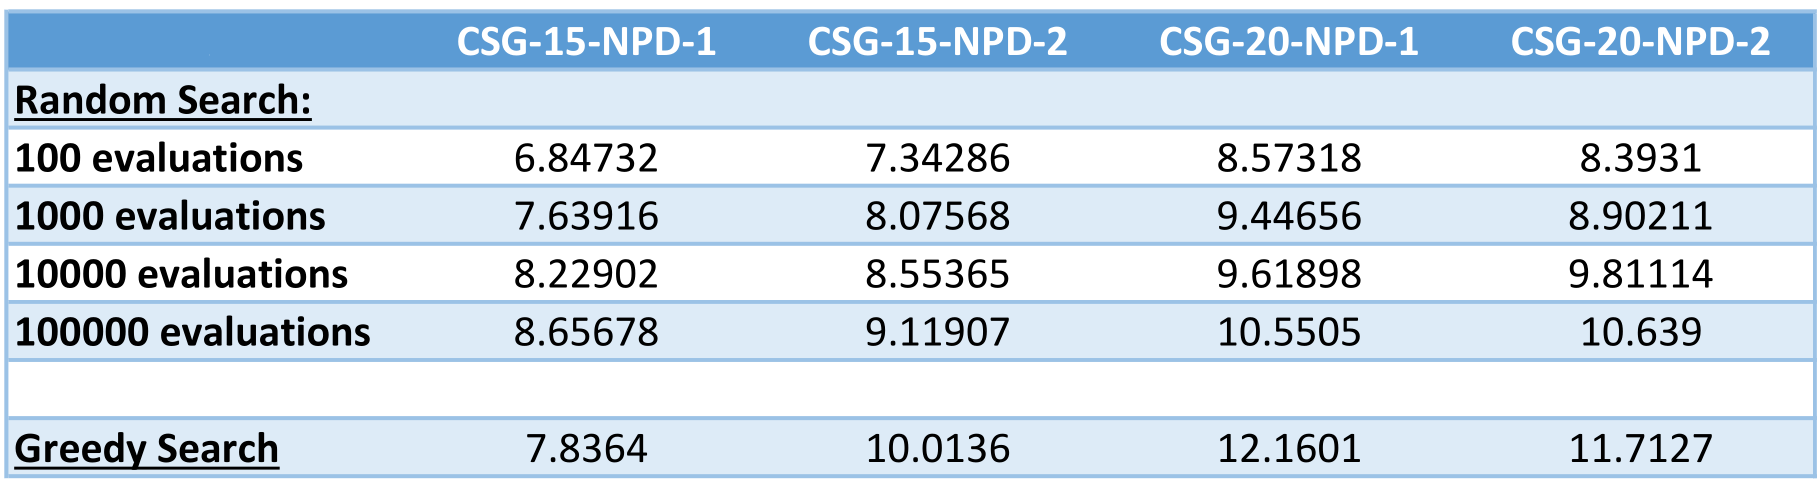
\includegraphics[width=\linewidth]{csg_data.png}
 \caption{Data obtained from the coalition structure generation exercise.}
 \label{fig:csg_data}
 \end{figure}

 The data plotted from these experiments in Figure \ref{fig:csg_graph} shows the global
  tendency from the results of the two algorithms. It can be very well seen that for the
  \textbf{Random Search} algorithm, the more evaluations we have, the better the utility
  value. It seems logical since there is more chance to have a better result. As for the
  \textbf{Greedy Search}, overall it seems to outperform the \textbf{Random Search}, but
  it looks like the more agents there are, the better it is in comparison. Which is also
  logical since, as the complexity increases (i.e. the number of solutions), one can expect 
  a random algorithm to have greater difficulties to find a very good solution than a
  structured algorithm.

 \begin{figure}[ht!]
 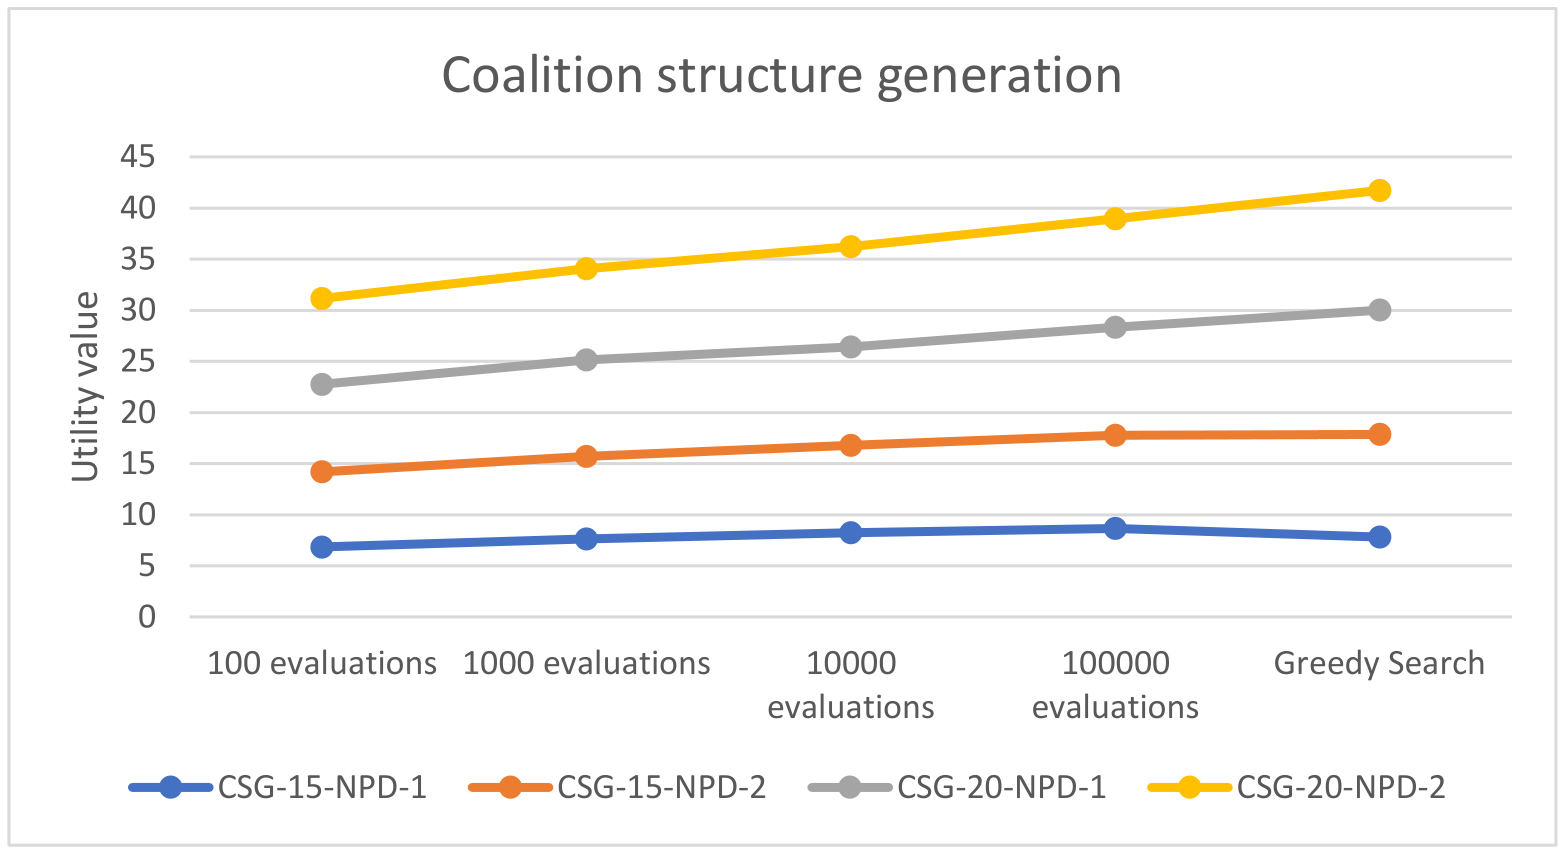
\includegraphics[width=\linewidth]{csg_graph.png}
 \caption{Utility values plotted with their relative algorithms and number of evaluations.}
 \label{fig:csg_graph}
 \end{figure}

 Thus, for a small problem, the \textbf{Random Search} can be more suitable complexity
  and computationally wise. Whereas the \textbf{Greedy Search} should be privileged for
  bigger problems.

\subsection*{2) \textbf{ Exercise 2: Coordinating coalitions}}
\textit {You should plot and discuss your results in the lab report from
 benchmarking the algorithms with the following problem sets.} \medskip

 This problem is a bit different since it is not the number of agents which increases from
  problems 1 \& 2 to problems 3 \& 4 but the number of \emph{task}. The results of our 
  implementation of the two algorithms are presented in Figure \ref{fig:scsga_data}.
  Looking at the results, we can observe that \textbf{Greedy Search} is systematically
  better than \textbf{Random Search} for as much as 100 000 evaluations.

 \begin{figure}[ht!]
 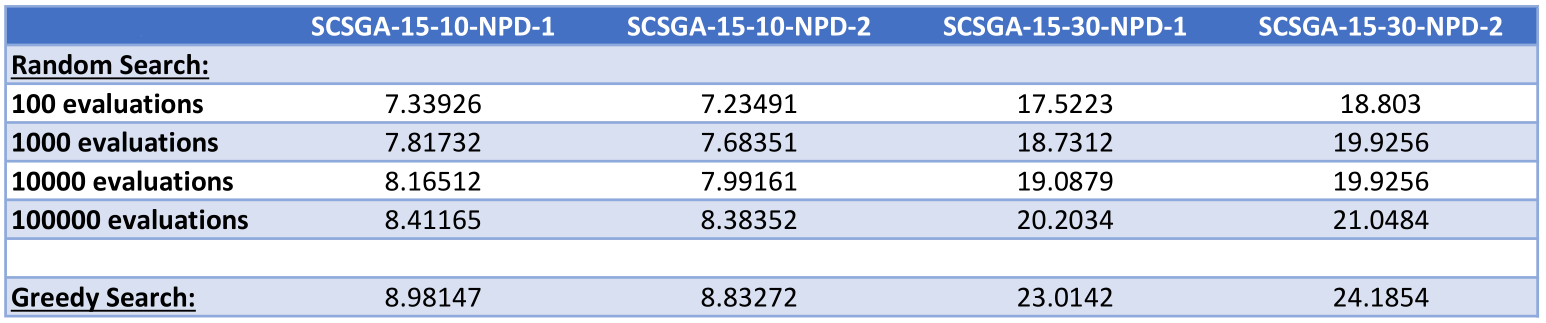
\includegraphics[width=\linewidth]{scsga_data.png}
 \caption{Data obtained from the Coordinating coalitions exercise.}
 \label{fig:scsga_data}
 \end{figure}

 By plotting the results in Figure \ref{fig:scsga_graph}, we can find the same tendency
  as for \textbf{Exercise 1}. Indeed, the \textbf{Greedy Search} seems to produced results
  a bit better than \textbf{Random Search} for smalls numbers of tasks, whereas the results
  difference is greater for a greater number of tasks.

 \begin{figure}[ht!]
 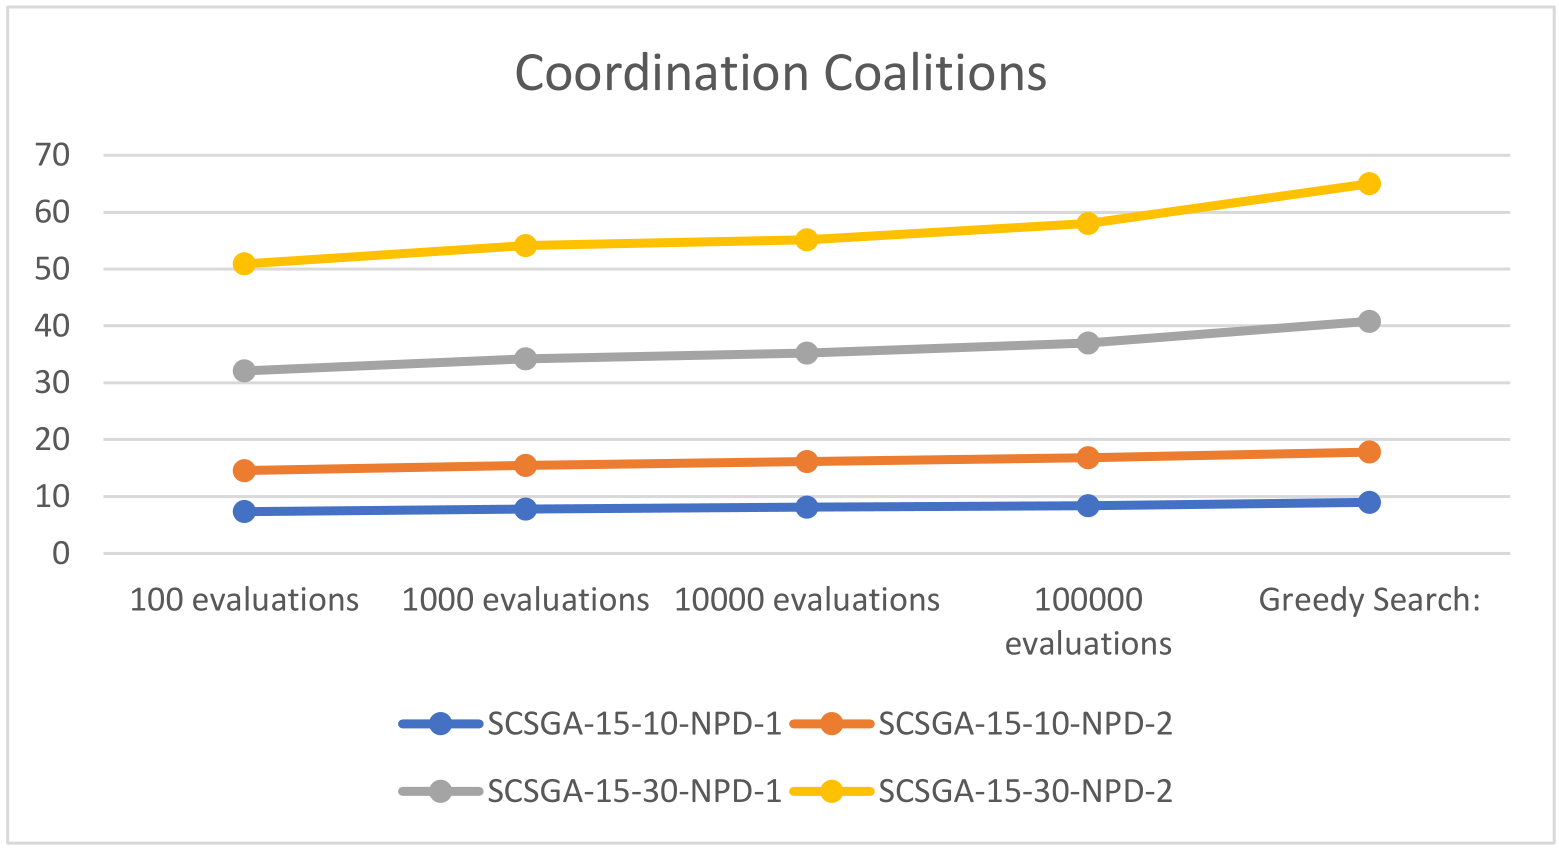
\includegraphics[width=\linewidth]{scsga_graph.png}
 \caption{Utility values plotted with their relative algorithms and number of evaluations.}
 \label{fig:scsga_graph}
 \end{figure}

In conclusion, for smalls numbers of tasks, the \textbf{Random Search} seems to be good
 enough but not the best, it can be again chosen for complexity or computational reasons.
 For larger number of tasks though, the \textbf{Greedy Search} will be better and better,
 hence should be privileged.   

\end{document}  
%%%%%%%%%%%%%%%%%%%%%%%%%%%%%%%%%%%%%%%%%%%%%%